\documentclass[a4paper]{article}
\usepackage[utf8]{inputenc}
\usepackage[german]{babel}
\usepackage{graphicx}
\usepackage{amsmath}
\usepackage{geometry}

\begin{document}
	\title{Versuchsprotokoll}
	\tableofcontents
	\newpage
	\section{Schallgeschwindigkeit in Gasen}
	\subsection{Kalibration des Potentiometers zur Streckenmessung}
	\label{section:Kalibration_Poti}
	\subsubsection{Versuchsbeschreibung}
	Zur Längenmessung soll ein Potentiometer eingesetzt werden. Dazu muss bei verschiedenen Auslenkungen der Widerstand R des Potentiometers gemessen werden und der entsprechenden Strecke s zugeordnet werden.\\
	
	Für den Widerstand des Potentiometers gilt:
	\begin{equation}
	R = R_0(1-\frac{x}{L})
	\end{equation}
	Der Regelbare Widerstand ist linear in der Auslenkung x innerhalb des Potentiometers, welche wiederum linear zu der von uns verwendeten Strecke s ist.\\
	
	Für die folgenden Versuche sind immer nur Streckendifferenzen $\Delta s$ von Interesse. Deswegen suchen wir den Umrechnungsfaktor k:
	\begin{equation}
	k = \frac{\Delta s}{\Delta R}
	\end{equation}
	Dieser entspricht offensichtlich der Steigung der Geraden durch die Messpunkte (R, s).
	
	\subsubsection{Versuchsaufbau und - durchführung}

	Vom Mikrofon aus läuft ein Seil über eine Umlenkrolle am Potentiometer, die den Widerstand reguliert. Am Ende des Seils, das hinter der Rolle nach unten hängt, befindet sich ein Gewicht, um guten Kontakt zwischen Seil und Rolle sicherzustellen. Der Widerstand R des Potentiometers wird mithilfe der Stromquellen-Box des CASSY Sensor Systems gemessen und gegen die aktuelle Position des Mikrofons aufgetragen. Als Rauschmessung für den Widerstand haben wir die Messung aus dem Versuch zur Laufzeitmessung (Kapitel \ref{section:Laufzeitmessung}) genutzt, da wir bei dieser Messung jeweils ca 20 Werte aufgenommen haben.\\
	
	\begin{tabular}{l l l}
		
		CASSY & Kanal B & Stromquellen-Box, Rb1 0-10kOhm Momentanwert \\ 
		 
		Messparameter & manuell &  7 Messungen\\ 
		
	\end{tabular} 
	
	\subsubsection{Versuchsauswertung}
	Der Fehler auf die Strecken ist jeweils durch den Ablesefehler sowie den Kalibrationsfehler des Maßbands gegeben.
	\begin{equation}
	\sigma _{stat} = 0,05 cm / \sqrt{12} = 0,15 cm \text{\qquad} \sigma_{sys} = 0,07 cm / \sqrt{3} = 0,04 cm
	\end{equation}

	An diese Rohdaten wurde eine Gerade angepasst. Die Steigung dieser Geraden mit $s=k\cdot R+b$ entspricht dem gesuchten Umrechnungsfaktor $k$.\\\\
	Aus der linearen Regression ergibt sich: $ k = (-15,99 \pm 0,07) \frac{cm}{k\Omega}$\\
	Das $\chi^2/dof = 1,012$ zeigt eine sehr gelungene Kalibration.
	\begin{center}
        \begin{tabular}{|c|c|}
        	\hline
	        \textbf{Strecke [$cm$]} & \textbf{Widerstand [$k\Omega$]} \\
	        \hline
	        10 & 2,375 \\
			\hline
			15 & 2,065 \\
			\hline
			20 & 1,765 \\
			\hline
			25 & 1,435 \\
			\hline
			30 & 1,12 \\
			\hline
			35 & 0,81 \\
			\hline
			40 & 0,505 \\
			\hline		
		\end{tabular}
	\end{center}
	\begin{center}
		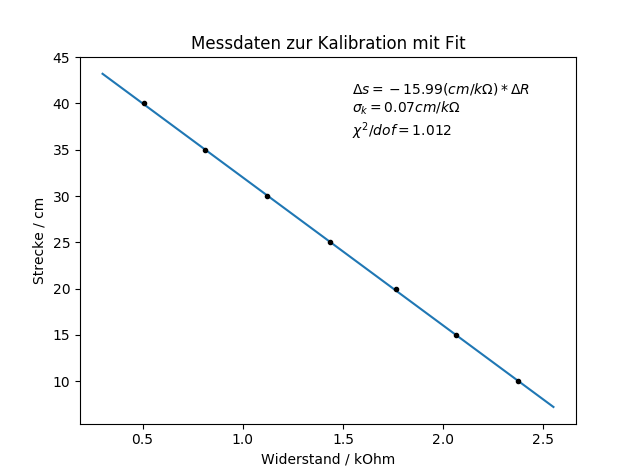
\includegraphics[width=0.7\linewidth]{kalibration_poti_fit}
	\end{center}
		
	
	
	\subsection{Laufzeitmessung}
	\label{section:Laufzeitmessung}
	\subsubsection{Versuchsbeschreibung}
	Schallwellen breiten sich in Gasen (z.B. Luft) mit begrenzter Geschwindigkeit $v_{Schall}$ aus. Um  $v_{Schall}$ zu bestimmen, wird in diesem Versuch direkt die Zeit gemessen, die der Schall für die Ausbreitung vom Lautsprecher bis zum Mikrofon benötigt.\\
	Es ist bekannt, dass in idealen Gasen gilt:
	\begin{equation}
	v_{Schall} = v_0 \sqrt{T/T_0} \text{\qquad mit \qquad} v_0 = \sqrt{\frac{R\cdot\kappa}{M_{mol}}T_0}
	\end{equation}
	Trägt man die Strecke $x$ gegen Laufzeit $t$ auf, so ergibt sich $v_{Schall}$ als Steigung der Geraden durch die Messwerte ($v=\frac{\Delta s}{\Delta t}$).
	
	\subsubsection{Versuchsaufbau und -durchführung}
	
	\begin{figure}
		\begin{center}
		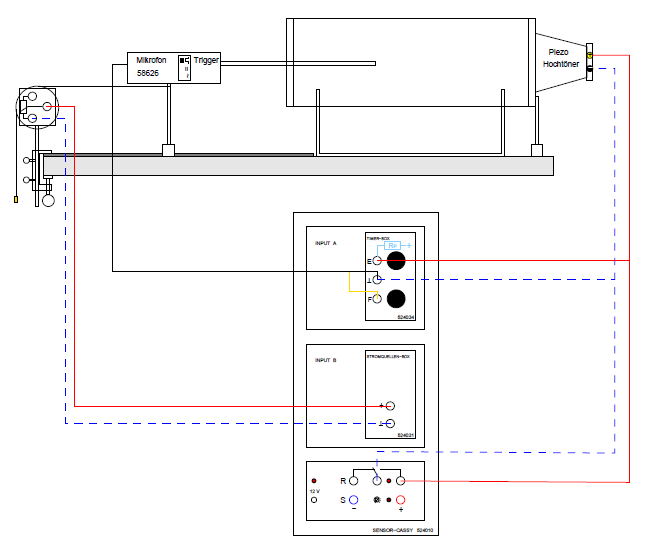
\includegraphics[width=0.7\linewidth]{aufbau_laufzeitmessung}
		\caption{CASSY Messaufbau: Laufzeit gegen Laufstrecke (Quelle: Praktikumsskript S. 38)}
		\label{pic:aufbau_laufzeit}
		\end{center}
	\end{figure}
	

	Als Lautsprecher wird ein Piezo-Hochtonlautsprecher verwendet. Dieser wird vom Relais - Schalterpaar R2/R3 des Sensor CASSY angesteuert. Diese liefern auch das Triggersignal zum Starten der Zeitmessung und das Mikrofon im Triggermodus gibt das Signal zum Beenden der Zeitmessung. Das Mikrofon steht verschiebbar auf einer Metallschiene, die mit einer Tischklemme am Ende des Tisches befestigt ist. Dort befindet sich auch ein Potentiometer (Stromquellenbox, Kanal B) mit Umlenkrolle, um Änderungen der Strecke Lautsprecher - Mikrofon aufzunehmen (siehe Kapitel \ref{section:Kalibration_Poti}). Am Ende der Metallschiene befindet sich eine Rohrhalterung mit Rohr, in dem die Messung stattfindet, um Störungen zu vermeiden. Abbildung \ref{pic:aufbau_laufzeit} zeigt den Aufbau. Außerdem wird die Lufttemperatur im Raum gemessen, um die theoretische Vorhersage für die Schallgeschwindigkeit zu ermitteln.\\\\
	Um die Schallgeschwindigkeit zu berechnen, wird die Laufzeit bei unterschiedlichen Mikrofonabständen gemessen. Wir haben je Abstandseinstellung ca. 20 Messwerte aufgenommen, um den statistischen Fehler auf die Messungen zu bestimmen. Dabei ist zu beachten, dass das Potentiometer einen Abstand Mikrofon - Potentiometer liefert. Das bedeutet:
	\begin{equation}
	\Delta s_{Lautsprecher-Mikrofon} = - \Delta s_{Mikrofon-Poti}	
	\end{equation}

		\begin{tabular}{l l l}
			CASSY & Kanal A & Laufzeit Dta1 E$\rightarrow$F, 0.002s, Flanken invertiert \\
			&Relais & frac(time)<0.1\\
			Messparameter & automatisch Intervall 1s \\
			& neue Messreihe anhängen
		\end{tabular}

	
	\subsubsection{Versuchsauswertung}
	
	Zunächst wurden die einzelnen Messreihen (Abbildung \ref{pic:messreihen_laufzeit}) auf statistische Fehler untersucht. Daraus ergab sich als Fehler für die Einzelmessungen:
	\begin{equation}
	\sigma _{R_{stat}} = 0,63 k\Omega \text{\qquad sowie \qquad} \sigma_{t_{stat}} = 0,29 ms
	\end{equation}
	Als systematischer Fehler auf die Widerstandsmessung der Stromquellen-Box haben wir ca. 1\% angenommen: 
	\begin{equation}
	\sigma_{R_{sys}} = 0.01 k \Omega
	\end{equation}
	\begin{figure}
	\begin{center}
		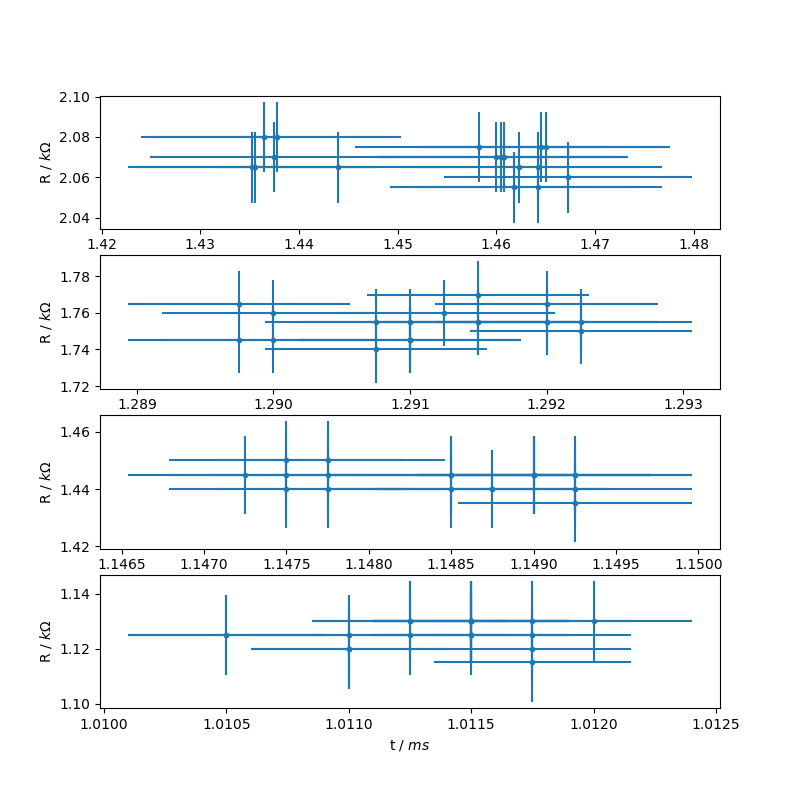
\includegraphics[width=0.6\linewidth]{messreihen_2bis5_laufzeit}
		\caption{Messreihen 2 bis 5 von insgesamt sieben Messreihen}
		\label{pic:messreihen_laufzeit}
		
		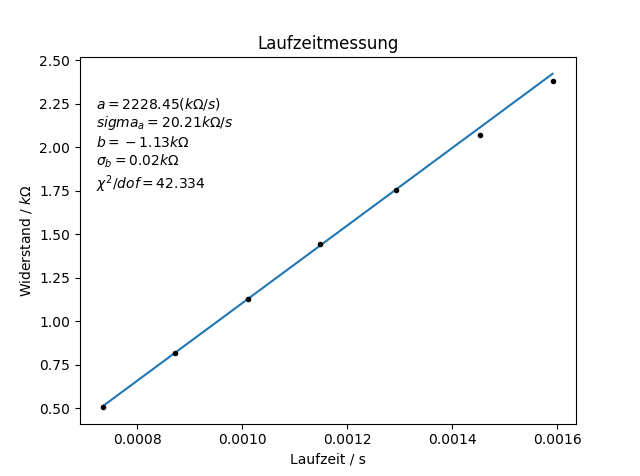
\includegraphics[width=0.6\linewidth]{fit_laufzeit}
		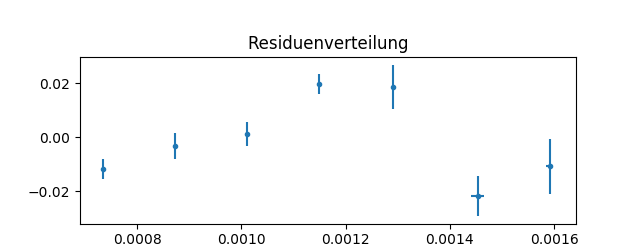
\includegraphics[width=0.6\linewidth]{residuen_laufzeit}
		\caption{Mittelwerte der Messreihen mit angepasster Geraden durch die Messwerte}
		\label{pic:fit_laufzeit}
		
		
	\end{center}
	\end{figure}
	An alle Messreihen zusammen wurde eine Gerade angepasst (Abbildung \ref{pic:fit_laufzeit}), es ergab sich für deren Steigung:
	\begin{equation}
	\frac{\Delta R}{\Delta t} = (2181,55 \pm 22,77) \frac{k\Omega}{s}
	\end{equation} 
	Gesucht ist die Schallgeschwindigkeit $v_{Schall}$, diese ergibt sich als Steigung der Geraden an die Messwerte, wobei die Widerstände noch in Entfernungen umgerechnet werden müssen. Da nur die Steigung von Interesse ist und nicht der y-Achsenabschnitt, wurde die tatsächliche  Entfernung Lautsprecher - Mikrofon weder gemessen noch berechnet. Es gilt:
	
	\begin{equation}
	v_{Schall} = \frac{\Delta s}{\Delta t} = \frac{\Delta s}{\Delta R} \cdot \frac{\Delta R}{\Delta t} = k \frac{\Delta R}{\Delta t} = 352,11 \frac{m}{s}
	\end{equation}
	\begin{equation}
	\sigma_{stat} = v_{Schall} \frac{\sigma _{\Delta R / \Delta t}}{\Delta R / \Delta t} = 3,64 \frac{m}{s}
	\end{equation}
	\begin{equation}
	\sigma_{sys} = v_{Schall} \frac{\sigma _k}{k} = 1,53 \frac{m}{s}
	\end{equation}
	
	Also ergibt sich als Ergebnis des Versuchs: $v_{Messung} = (348,90 \pm 3,64 \pm 1,53) \frac{m}{s}$. \\\\
	Aus der Temperaturmessung erhielten wir, dass die Raumtemperatur zu Beginn des Versuchs $T = (23,459 \pm 0,001)C = (296,609 \pm 0.001)K$ betrug.
	Daraus ergibt sich eine Schallgeschwindigkeit von
	\begin{equation}
	v_{Theorie} =\sqrt{\frac{R\cdot\kappa}{M_mol}}\sqrt{T} = 345,1398 \frac{m}{s} \text{\qquad mit \qquad}
	\sigma = 0,5 \sqrt{\frac{R\cdot\kappa}{M_mol}} \frac{\sigma_T}{\sqrt{T}} = 0,00058 \frac{m}{s}
	\end{equation}
	Die Abweichung der Messung von der Theorie beträgt demnach 0,73 Standardabweichungen. Damit ist die Messung im Rahmen der angegebenen Unsicherheit nah am erwarteten Wert. Die relative Unsicherheit auf die Schallgeschwindigkeit beträgt 1,48\%, was durchaus ein guter Wert ist.
	
	Die Geradenanpassung ergibt mit einem $chi^2/dof = 2,08$, dass die Fehler tendenziell noch etwas zu klein abgeschätzt wurden.
	\begin{table}
		\begin{center}
			\begin{tabular}{|c|c|}
				\hline
				\textbf{Widerstand [$k\Omega$]} & \textbf{Laufzeit [$s$]} \\
				\hline
				2.3792 & 0.001591 \\
				\hline
				2.0682 & 0.001453 \\
				\hline
				1.7535 & 0.001292 \\
				\hline
				1.4435 & 0.001148 \\
				\hline
				1.126 & 0.001011 \\
				\hline
				0.8178 & 0.0008721 \\
				\hline
				0.5075 &  0.0007338 \\
				\hline
			\end{tabular}
		\end{center}
		\caption{Mittelwerte der Messreihen}
	\end{table}
	
\end{document}